\section{Introduction}
% Trombetta: Most of what I have is not running shin splints stuff; hopeful you found some there. I do have some general human running stuff in the list. You might ask 1/C Anmol Walha about running biomechanics, and 1/C Lily Bautista about walking and ankles? I have their 485 projects but not the references they found... 
%Work from an inverted triangle (broader topics to more specific). Explain what you are interested, review some relevant literature, and then set up what your specific research question is. Cite literature using the author-year format, as in \citep{buck2020go}. If you need pictures to explain the relevant biomechanics, feel free to include. This section should also say a little why your research matters. The last part of this section should be the specific hypotheses you seek to test. 

%What is shin splint? 
%To study the effectiveness and injury risk of heel strike versus forefoot strike running.
\citet{slocum1967shin} medically described shin splints as a symptom complex characterized by pain and discomfort in the lower leg after repetitive overuse in walking or running. The usual sites of pain are the lower half of the posteromedial border of the tibia, the anterior tibial compartment, the tibia, and the interosseous membrane; other additional technical details are provided to distinguish it from stress fractures, anterior tibial syndrome, and muscle hernia \citep{slocum1967shin}. As a midshipman in my first year at the United States Naval Academy, I am acutely familiar with repetitive overuse of the lower leg in walking and running, which motivates me to understand how biomechanics may play a role in avoiding shin splints. 

\subsection{Potential for running style to reduce risk of shin splints}
%Explain heel strike versus forefoot strike
One potential avenue to reduce shin splints is running style. Heel-strike is a style in which the initial contact of the foot with the ground, at the beginning of the stance phase, is made using the heel. In contrast, forefoot-strike involves using the ball of the foot or other midfoot parts. Popular press articles for runners discuss the potential for running style in reduce or prevent injuries \citep{douglas2012midfoot, giandolini2013impact}, while the general biomechanics of running is reviewed in \citep{chan1994foot, lieberman2020biomechanical, bramble2004endurance, lieberman2010foot}. 

What is the evidence that suggests forefoot-strike and similar styles might help with shin splints? \citet{larson2014comparison} examined barefoot and minimally shod runners in a recreational road race and found only 20.7\% of barefoot runners were rearfoot (heel) strikers. \citet{gans1985relationship} studied ballet dancers and found that dancers with a history of shin splints demonstrated more double heel strikes when executing a sequence of jumps. In an Army study, \citet{diebal2012forefoot} found a 6-week forefoot strike running intervention reduced pain and disability associated with chronic exertional compartment syndrome. \citet{willems2004intrinsic} conducted a study with 400 physical education students and found subjects that developed exercise-related lower leg pain had an altered running pattern compared to the controls including a more central heel strike. 

On the other hand, \citet{cibulka1994shin} presented a case study of a patient with shin splints who ran using a forefoot contact running style, whose symptoms were resolved when shifting to a heel-toe style. In another Army study, \citet{warr2015characterization} characterized foot-strike patterns in 341 soldiers and found no difference between injury rates or performance on a two-mile run between heel-strike and nonheel-strike. \citet{thacker2002prevention} states that use of shock-absorbent insoles, foam heel pads, heel cord stretching, alternative footwear, as well as graduated running programs among military recruits have undergone assessment in controlled trials, which have not shown strong support for any of these interventions. \citet{thacker2002prevention} concluded that the literature yielded little objective evidence to support widespread use of any existing interventions to prevent shin splints, and suggested a rigorously implemented research program is critically needed to address this common sports medicine problem.




\subsection{Are there observable biomechanical differences between running styles that may reduce the risk of shin splints?}

My guiding research question is, what relevant and quantitaive biomechanics observations can I make regarding between running styles?  While the global COVID-19 pandemic limited my access to lab instrumentation, studies of human running gait and biomechanics historically made use of clever improvised methods to provide insight \citep{baker2007history, mcmahon1984muscles, mayer2010physiological, marey1873locomotion, carlet1872essai, muybridge1901human}. In particular, early studies made groundbreaking use of photography \citep{muybridge1901human, baker2007history, mcmahon1984muscles, mayer2010physiological} and wearable instrumentation \citep{marey1873locomotion, carlet1872essai, baker2007history, mayer2010physiological}. The wearable instrumentation available to early researchers (\fref{fig:intro}) included the kymograph, in which movement of limbs or pressure of the feet, transmitted via tubes or mechanical linkages, were use to actuate a stylus and inscribe records of force or motion, for example, on a soot blackened glass slide or cylinder. More modern versions of this instrumentation have been used as a cheap way to record maximal flows and forces for instrumentation deployed in the intertidal zone in heavy California surf \citep{bell1984quantifying, denny1983simple}.
\begin{figure}
\begin{center}
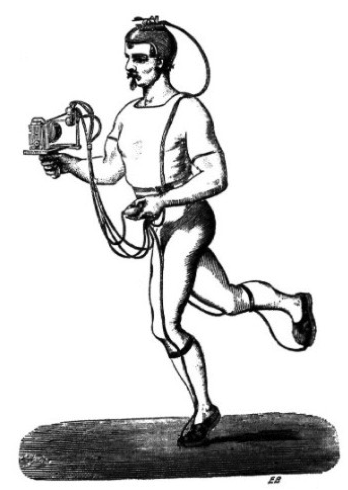
\includegraphics[height=1.5in]{figures/intro3.png}\hspace{0.5in}
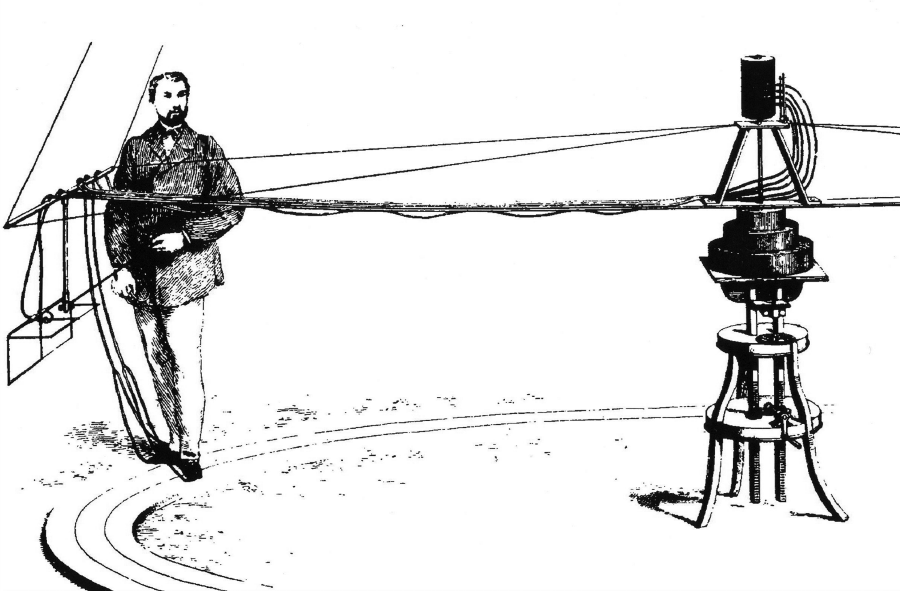
\includegraphics[height=1.5in]{figures/intro4.png}
\end{center}
\caption{Early wearable instrumentation applied to running biomechanics, from \citep{marey1873locomotion, carlet1872essai}. Tubes, mechanical linkages, and other contrivances were used to actuate a stylus, providing a record of stride frequency, angles, forces, or other data.} 
\label{fig:intro}
\end{figure}

I hypothesize that the apparent reduced risk of shin splints in forefoot strike / toe-strike could be due to lower overall forces or accelerations, as measured using a force plate or wearable accelerometer. Alternatively, the overall forces and accelerations may be similar between the two styles, but may have fine kinematic details that suggest a mechanism for clinical observations regarding running style. 



